\chapter{Results}\label{sec:results}
% In this chapter we expect you to list and explain all the results that you have achieved. Pictures can be useful to explain the results. Think about this chapter as something similar to the demo of the oral presentation. You can also include pictures about use-cases (you can also decide to add use cases to the high level overview chapter).

\section{Testing of the CamPUF}
The effectiveness and reliability of the CamPUF implementation were thoroughly evaluated through a comprehensive testing process. This section presents the details of the dataset used for testing, the setup of the testing environment, and the expected results. Additionally, the outcomes of the testing process will be presented, showcasing the algorithm's performance in various scenarios.

\subsection{Dataset}\label{sec:dataset}
After some testing, this dataset was eventually chosen \cite{dataset}. It is composed of various sets of both RAW and JPEG images taken with five different 12-megapixel Sony IMX377 camera sensors, used by Google Nexus 5X smartphones. The key aspect in the preference of this dataset over the others tested is that all the RAW images are completely dark photos taken with the sensor lens fully covered. This is critical since the DSNU extraction efficiency is highly influenced by the presence of any light source exposed to the sensor. [Figure \ref{fig:dataset}]

Another advantage of choosing this dataset is that it was made with the purpose of testing another CamPUF implementation, having different relevant configuration ready to test, as for images taken in different room temperatures ($25^{\circ}$C, $35^{\circ}$C and $45^{\circ}$C). It is worth noting that for any real-world practical implementation, the images provided to the enrollment/authentication algorithm should be taken in a similar way, in RAW format and trying to cover the sensor lens as much as possible.

\begin{figure}[h!]
	\vspace{0.5cm}
	\centering
	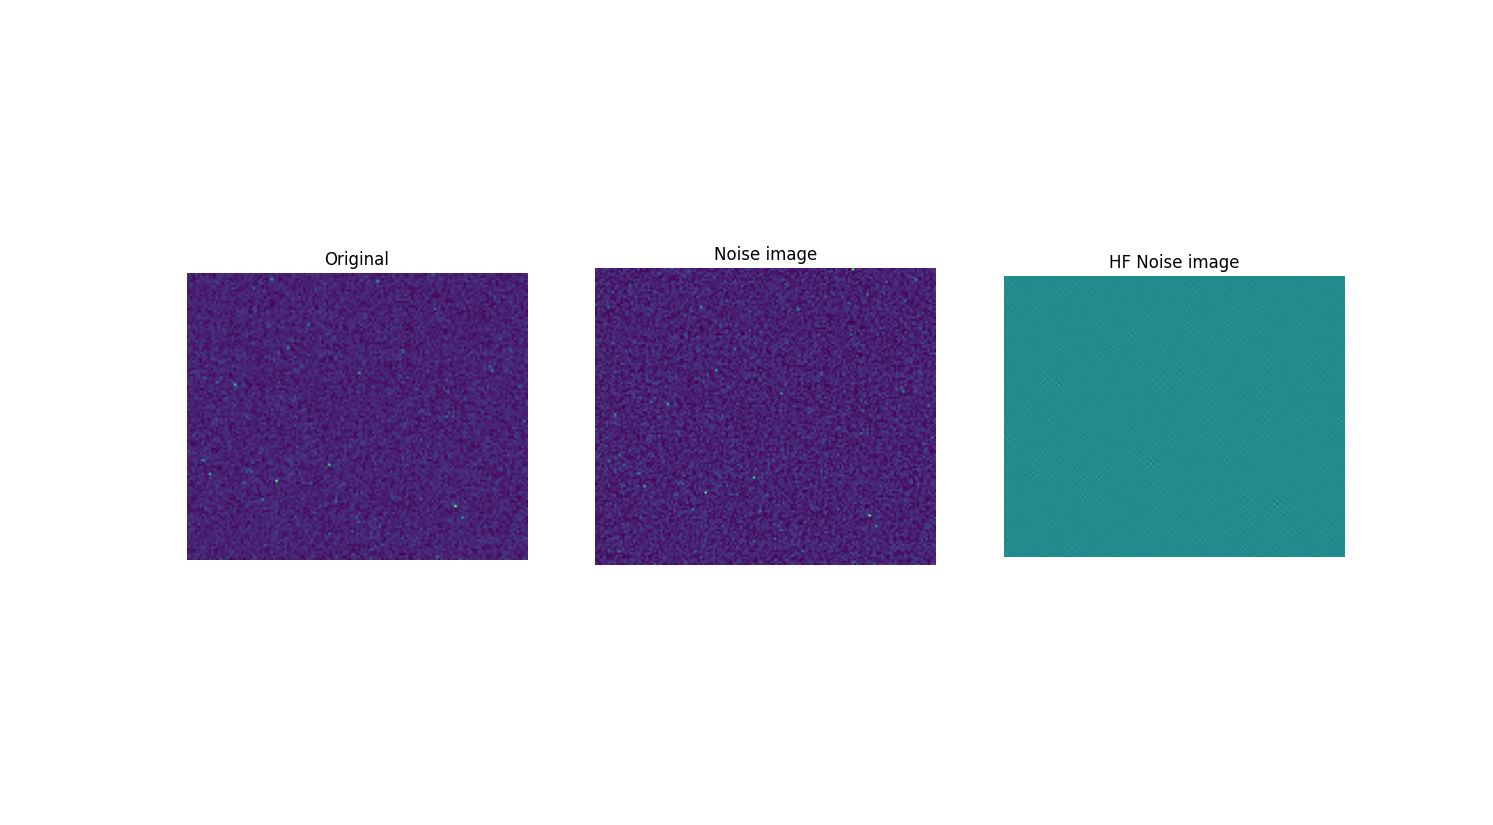
\includegraphics[width=\textwidth]{images/DSNU_S2S1I1.png}
	\caption{Example of DSNU extraction from one image of the dataset.}
	\label{fig:dataset}
\end{figure} 

\subsection{Setup}
The dataset was then thoroughly tested using a python script \emph{auto\_testing.py} that automated the following steps:

\begin{enumerate}
	\item Reading one or multiple images (and in this case, making the pixel-wide average).
	\item Obtaining the reference key after enrolling with that image.
	\item Trying to authenticate with a set of images, one after the other, by comparing the response key with the reference key generated from the previous step. If the Hamming Distance of the two keys is below a certain threshold, then the couple (\emph{enrollment image}, \emph{authentication image}) is said to be authenticated.
	\item After trying all the images combinations, the script computes the Hamming Distance average for the couple (\emph{enrollment image}, \emph{authentication set}).
\end{enumerate}

The main difference when picking the \emph{authentication set} to use is the source sensor of the images with respect to the source sensor of the \emph{enrollment image}. Two different cases are distinguished:

\begin{itemize}
	\item \textbf{Intra-Sensor} testing: both the \emph{enrollment image} and the \emph{authentication set} come from the same source sensor.
	\item \textbf{Inter-Sensor} testing: The \emph{enrollment image} and the \emph{authentication set} come from a different sensor.
\end{itemize}

\subsubsection{Parameters}
The main parameters used were generally:
\begin{itemize}
	\item \textbf{Key Length}: 256 bits, both for the reference key and the response key.
	\item \textbf{Hamming Distance Threshold}: 4 bits.
	\item \textbf{Number of Frames Averaged}: 5 frames for the enrollment, 1 frame for the authentication.
	\item \textbf{Number of Images tested for Authentication}: generally 50 for each run, 20 in the case of temperature testing. [Chapter \ref{sec:temperature}]
\end{itemize}

\subsubsection{Expected Results}

For the algorithm to be of any use, when testing \textbf{Intra-Sensor} couples it is expected to yield positive results on the authentication, meaning that the \emph{Intra-Sensor Hamming Distance} between the reference key and the response key must be low enough, ideally zero. This is needed in order to avoid any false negatives where devices are incorrectly unauthorized.

Another crucial assumption is related to the opposite case, where \textbf{Inter-Sensor} couples are expected to yield negative results on the authentication, meaning that the \emph{Inter-Sensor Hamming Distance} between the reference key and the response key must be high enough, in this case ideally around 50\% of the key length to match the expected Hamming Distance of two random bit sequences. Finally, this is also needed to avoid any false positives where devices are incorrectly authorized.

\subsection{Results}
The results were gathered after several runs of the \emph{auto\_testing.py} script. The results obtained from the testing process are in line with the expected outcomes, validating the effectiveness of the CamPUF implementation. The graph below presents the Hamming Distance percentages for different scenarios, considering 1 frame and 5 frames for both \textbf{Intra-Sensor} and \textbf{Inter-Sensor} testings:

\begin{figure}[h!]
	\centering
	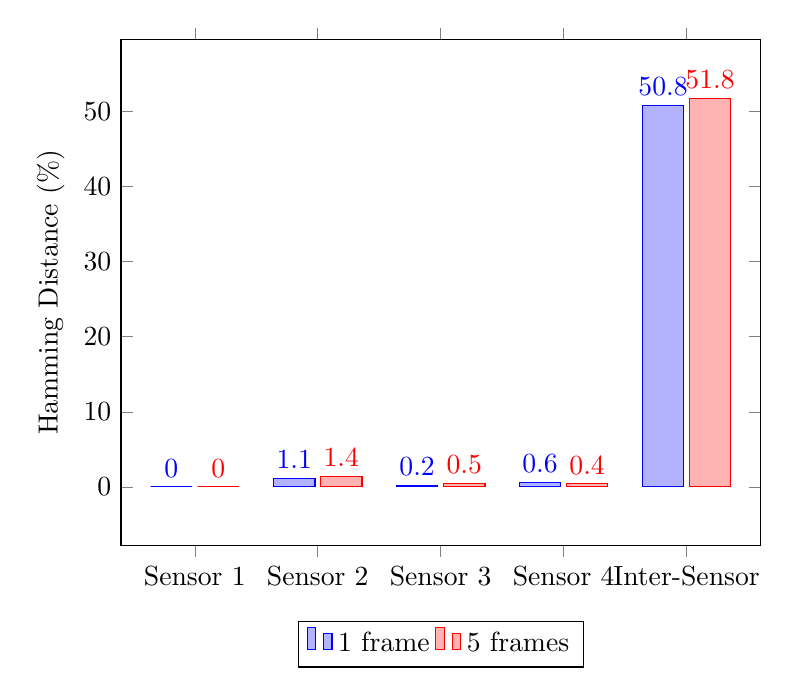
\begin{tikzpicture}
		\begin{axis}[
			width=0.8\textwidth,
			height=8cm,
			bar width=15pt,
			ybar,
			enlargelimits=0.15,
			legend style={at={(0.5,-0.15)},
			anchor=north,legend columns=-1},
			ylabel={Hamming Distance (\%)},
			symbolic x coords={Sensor 1, Sensor 2, Sensor 3, Sensor 4, Inter-Sensor},
			xtick=data,
			nodes near coords,
			nodes near coords align={vertical},
			]
			\addplot coordinates {(Sensor 1, 0.0) (Sensor 2, 1.1) (Sensor 3, 0.2) (Sensor 4, 0.6) (Inter-Sensor, 50.8)};
			\addplot coordinates {(Sensor 1, 0.0) (Sensor 2, 1.4) (Sensor 3, 0.5) (Sensor 4, 0.4) (Inter-Sensor, 51.8)};
			\legend{1 frame, 5 frames}
		\end{axis}
	\end{tikzpicture}
	\caption{Hamming Distance Percentages for Intra-Sensor and Inter-Sensor Testings}
	\label{fig:results_graph}
\end{figure}

As evident from the graph in Figure \ref{fig:results_graph}, the CamPUF algorithm performed exceptionally well in \textbf{Intra-Sensor} testing. Even with just one image for enrollment, the Hamming Distance between the reference key and the response key was found to be remarkably low. This demonstrates that a single image is sufficient to achieve accurate intra-sensor authentication, showcasing the efficiency of the algorithm.

Moreover, it was observed that a relatively low threshold of 4 bits is adequate to determine authentication success. This means that if the Hamming Distance falls below the threshold, the authentication process is successful. Fine-tuning this threshold allows for balancing between security and convenience. Lowering the threshold can increase security but may require more attempts to successfully authenticate. Conversely, increasing the threshold may reduce security but lead to faster and easier authentication.

The \textbf{Inter-Sensor} testing results align with expectations, showing Hamming Distances around 50\%, which is in line with the expected Hamming Distance between two random bit sequences. This confirms that CamPUF effectively discriminates between images taken from different sensors, providing a reliable mechanism to prevent unauthorized access.

\subsubsection{Temperature Resilience}\label{sec:temperature}

One critical aspect of the CamPUF implementation is its resilience to changes in temperature, which can impact the quality of sensor outputs. Higher temperatures often lead to increased random noise coming from the electrons inside the CMOS sensors, resulting in less noticeable DSNU noise that the algorithm relies on \cite{temperature}. We conducted testing under varying temperatures to assess the algorithm's performance in such scenarios.

The sensor tested for Intra-Sensor testing was Sensor 1, and the temperature changes refer to the room temperature relative to the images used for the authentication phase. The enrollment was always done with a room temperature of 25°C.

\begin{figure}[h!]
	\centering
	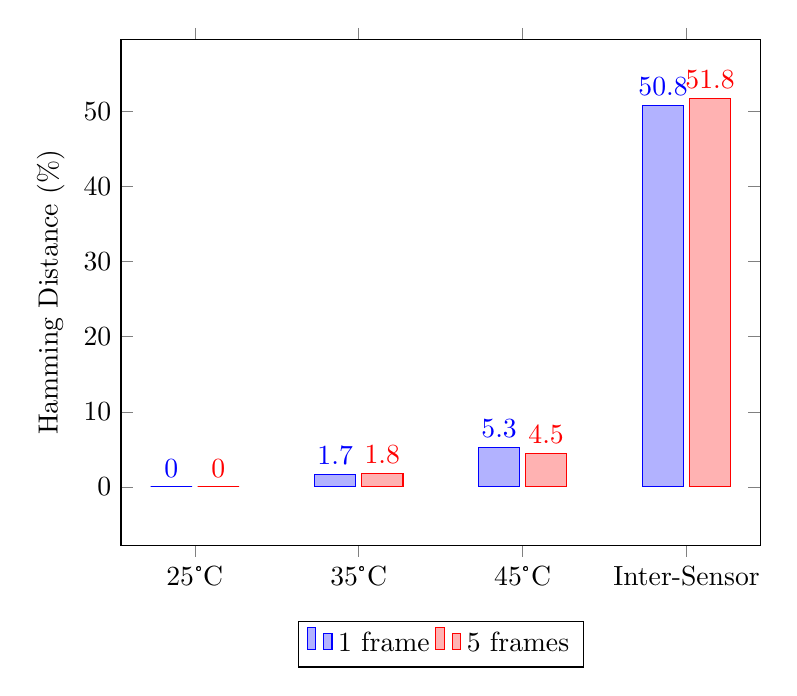
\begin{tikzpicture}
		\begin{axis}[
			width=0.8\textwidth,
			height=8cm,
			bar width=15pt,
			ybar,
			enlargelimits=0.15,
			legend style={at={(0.5,-0.15)},
			anchor=north,legend columns=-1},
			ylabel={Hamming Distance (\%)},
			symbolic x coords={25°C, 35°C, 45°C, Inter-Sensor},
			xtick=data,
			nodes near coords,
			nodes near coords align={vertical},
			]
			\addplot coordinates {(25°C, 0.0) (35°C, 1.7) (45°C, 5.3) (Inter-Sensor, 50.8)};
			\addplot coordinates {(25°C, 0.0) (35°C, 1.8) (45°C, 4.5) (Inter-Sensor, 51.8)};
			\legend{1 frame, 5 frames}
		\end{axis}
	\end{tikzpicture}
	\caption{Hamming Distance Percentages for Intra-Sensor and Inter-Sensor Testings at Different Temperatures}
	\label{fig:temperature_graph}
\end{figure}

As expected, the results in Figure \ref{fig:temperature_graph} show that the average Intra-Sensor Hamming Distance rises with increasing temperatures. At 25°C, the Hamming Distances remain negligible (0.0\%) for both one frame and five frames enrollments, indicating that even with minimal data, the algorithm achieves accurate authentication. However, at higher temperatures of 35°C and 45°C, the Intra-Sensor Hamming Distances slightly increase to 1.7\% and 5.3\% (for one frame enrollment), and 1.8\% and 4.5\% (for five frames enrollment), respectively.

Despite the slight increase in Intra-Sensor Hamming Distances with rising temperatures, they remain significantly low compared to the Inter-Sensor Hamming Distances, which are consistently around 50.8\% for one frame enrollment and 51.8\% for five frames enrollment. This highlights the algorithm's robustness and its ability to maintain reliable authentication even under varying temperatures.

\subsection{Shared Images Attacks Mitigation}\label{sec:attacks}

One important aspect to address when considering the security of CamPUF is the potential vulnerability to attacks where an attacker tries to authenticate using images taken from the victim sensor, if shared on platforms like social networks or the internet. However, the CamPUF implementation has inherent defense mechanisms that effectively mitigate these potential threats in two key ways:

\subsubsection{Difficulty of Obtaining Useful Images}

A fundamental aspect of the CamPUF enrollment process is the use of completely dark images with the sensor lens fully covered. This means that during enrollment, the CamPUF captures the sensor's unique noise pattern in the absence of any light sources. As a result, the enrollment phase requires acquiring and processing specific dark images, which are not commonly shared or readily available to the attacker. This rarity of sharing completely dark images limits attackers ability to obtain the specific enrollment images needed to replicate the CamPUF response.

\subsubsection{Impact of JPEG Compression}

Even if an attacker manages to acquire and share a dark image used for enrollment, the authentication process remains highly resistant to attacks due to JPEG compression. When images are shared on social networks or the internet, they are often subjected to JPEG compression, a lossy compression technique that reduces file size by discarding high-frequency components. \cite{jpeg}

In the context of CamPUF, this JPEG compression has a crucial impact on the DSNU extraction process. The noise pattern required for CamPUF authentication predominantly resides in the high-frequency components of the sensor images. However, during JPEG compression, these high-frequency components are significantly altered or discarded, rendering the compressed image practically unusable for the DSNU extraction process.

This can be observed in the difference between the high-frequency components of RAW and JPEG dark images [Figure \ref{fig:jpeg_comp}]. The JPEG-compressed image loses essential details, making it unsuitable for accurate DSNU extraction.

\begin{figure}[h!]
	\centering
	\vspace{0.5cm}
	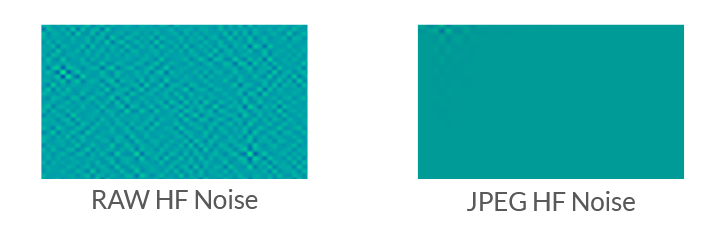
\includegraphics{images/jpeg_vs_raw_HF.png}
	\caption{Comparison of High-Frequency Components in RAW and JPEG Dark Images}
	\label{fig:jpeg_comp}
\end{figure}

As a result, if an attacker attempts to authenticate using a JPEG-compressed dark image, the Hamming distances observed in testing would be similar to the \emph{Intra-Sensor Hamming Distances}. In other words, the image is seen from the authentication algorithm as one coming from a different sensor, even if the original RAW image is from the same one used to enroll. This will lead to the JPEG image correctly not being authenticated, as expected.

\section{Known Issues}
% If there is any known issue, limitation, error, problem, etc...explain it in this section. Use a specific subsection for each known issue. Issues can be related to many things, including design issues.
The main limitation of this implementation of CamPUF is the need for a dataset of images highly similar to the one used for testing described in [Chapter \ref{sec:dataset}]. The CamPUF algorithm has demonstrated promising results using the specific dataset employed for testing.

While the dataset's characteristics, are crucial for efficient DSNU extraction, the algorithm's generalization to other datasets or real-world images remains uncertain. Variations in lighting conditions, exposure settings, and environmental factors in different image sources could influence the noise patterns and, in turn, impact the algorithm's authentication performance. 

Another important aspect is that newer sensors may exhibit different noise characteristics, including potentially lower DSNU components. This could affect the algorithm's ability to accurately extract the unique noise pattern necessary for device authentication.


\section{Future Work}
% Adding a section about how to improve the project is not mandatory but it is useful to show that you actually understood the topics of the project and have ideas for improvements.
\label{sec:future_work}

As the CamPUF implementation progresses towards real-world deployment, several key areas of focus for future work will enhance its performance, security, and practicality:

\subsubsection{Generalization to Different Sensors}

Efforts need to be made to extend the CamPUF implementation to work with a more diverse range of images beyond the current dataset, which mainly comprises completely dark photos with covered sensor lenses. The goal is to enhance the algorithm's versatility and ensure its effectiveness under real-world scenarios that involve various lighting conditions and newer sensors that could intrinsically attenuate the DSNU component needed for the PUF to work.

\subsubsection{On-Device Key Extraction Application}

To enable secure and efficient device authentication directly on devices, a dedicated on-device key extraction application needs to be developed. This application will be responsible for capturing a number of images and then processing the raw data from the sensor, extracting the DSNU, and generating the corresponding key.

\subsubsection{Server-Side Software}

A specific software also needs to be deployed to trusted servers that will implement the enrollment and authentication phase. This server-side application will securely store and manage the reference keys of enrolled devices and generate challenges for the authorization of devices.

\subsubsection{Fine-Tuning Parameters}

Parameters such as \emph{key length}, \emph{Hamming distance threshold}, and the \emph{number of frames} averaged during enrollment and authentication phases can be fine-tuned and optimized. The objective is to adapt the CamPUF to different scenarios to meet specific security requirements while still providing a seamless user experience. This can also be done with the help of Machine-Learning models capable of automatically adjust the parameters without the need of human intervention.

\subsubsection{Security Analysis}

While the main weakness of CamPUF, \emph{shared images} attacks, is described in [Chapter \ref{sec:attacks}], other areas of this implementation need to be evaluated to find other possible vulnerabilities.

\subsubsection{Real-World Integration \& Deployment}

The deployment process will involve integrating both the key extraction application and trusted server implementation into the target devices and server infrastructure. Additionally, integration of the CamPUF authentication mechanism with existing authentication systems and security frameworks can also be a focus point. Ensuring compatibility and interoperability with a wide range of devices and applications will increase its usability in real-world scenarios.